\documentclass[11pt, letterpaper]{article}

% Encoding
\usepackage[T1]{fontenc} % Output
\usepackage[latin1]{inputenc} % Input

% MATHS
\usepackage{amsmath, amssymb, amsfonts} % Math stuff
% linenofix -------------------------------------------
\newcommand*\patchAmsMathEnvironmentForLineno[1]{%
  \expandafter\let\csname old#1\expandafter\endcsname\csname #1\endcsname
  \expandafter\let\csname oldend#1\expandafter\endcsname\csname end#1\endcsname
  \renewenvironment{#1}%
     {\linenomath\csname old#1\endcsname}%
     {\csname oldend#1\endcsname\endlinenomath}}% 
\newcommand*\patchBothAmsMathEnvironmentsForLineno[1]{%
  \patchAmsMathEnvironmentForLineno{#1}%
  \patchAmsMathEnvironmentForLineno{#1*}}%
\AtBeginDocument{%
\patchBothAmsMathEnvironmentsForLineno{equation}%
\patchBothAmsMathEnvironmentsForLineno{align}%
\patchBothAmsMathEnvironmentsForLineno{flalign}%
\patchBothAmsMathEnvironmentsForLineno{alignat}%
\patchBothAmsMathEnvironmentsForLineno{gather}%
\patchBothAmsMathEnvironmentsForLineno{multline}%
}
%-----------------------------------------------------

\usepackage{mhsetup, mathtools, empheq} % Other optional maths stuff
\usepackage{mathrsfs}
\usepackage{amsthm}
\newenvironment{myproof}{\begin{proof}[\unskip\nopunct]}{\end{proof}}

% FORMATTING
\usepackage{array} % Tables etc
\usepackage{longtable} % Break table over pages
\usepackage{pdflscape} % to turn table in landscape mode

\usepackage{multirow} % Join cells over multiple rows
\usepackage{paralist} % In-paragraph itemized lists (\begin{inparaenum}\item.... \end{inparaenum})
\usepackage{lineno} % For line numbering
\usepackage{setspace} % Line spacing
\usepackage{nameref} % Reference to section name, not just number

\usepackage{chngcntr} % For equation counter in the appendix

% HEAD AND FOOT
\usepackage{fancyhdr}
\fancypagestyle{maintext}{
\fancyhf{}
\fancyhead[C]{}
\fancyfoot[C]{\thepage}
\renewcommand{\headrulewidth}{0.pt}
}

\fancypagestyle{appendix}{
\fancyhf{}
\fancyhead[C]{{\sf Appendix \thesection{}}}
\fancyfoot[C]{\thepage}
\renewcommand{\headrulewidth}{0.5pt}
}

% BIBLIOGRAPHY
\usepackage[]{natbib} % Package for the bibliography

% Colors
\usepackage[table]{xcolor}

% FIGURES
% Package to label the different panels of a figure
\usepackage[FIGTOPCAP, raggedright, sf, bf, scriptsize, SF, nooneline]{subfigure} 
% Tikz and related packages (to draw figures)
\usepackage{tikz}
\usetikzlibrary{positioning,shadows,arrows,trees, shapes, fit, calc}
% Style of the captions
\usepackage[font={small,sf, doublespacing}, labelfont=bf]{caption}


\usepackage{floatrow}

%% FONTS
% Fonts of the main text
\usepackage{fourier}
% Helvetica for sans serif fonts
\renewcommand{\sfdefault}{phv}
% Make sure mathcal looks the same
\DeclareMathAlphabet{\mathcal}{OMS}{cmsy}{m}{n}

% SECTIONS
\usepackage{titlesec}
\usepackage{needspace}

%% Section
\titleformat{\section}[block]
  {\needspace{2in}\Large \bfseries\sffamily}
  {\thesection}
  {1em}
  {}
% Subsection
\titleformat{\subsection}[block]
  {\large\bfseries\sffamily}
  {\thesubsection}
  {1em}
  {} 
% Subsubsection
\titleformat{\subsubsection}[block]
  {\bfseries\sffamily}
  {\thesubsubsection}
  {1em}
  {} 
% Paragraph
\titleformat{\paragraph}[runin]
  {\sffamily\normalsize\bfseries}
  {\theparagraph}
  {0em}
  {}

% TABLES
\usepackage{multirow}
\usepackage{rotating}

\usepackage[colorlinks=true, citecolor=black, linkcolor=black, urlcolor=black]{hyperref}
\hypersetup{
%    pdftitle={Mutation and social evolution},
 %   pdfauthor={Your name here},
 %   pdfsubject={Your subject here},
  %  pdfkeywords={keyword1, keyword2},
  %  bookmarksnumbered=true,     
    bookmarksopen=true,         
  %  bookmarksopenlevel=1,       
  %  colorlinks=true,            
    pdfstartview=Fit,           
    pdfpagemode=UseOutlines,    % this is the option you were lookin for
  %  pdfpagelayout=TwoPageRight
}


% STYLES IMPORTED FOR EQREF DOCUMENT
\makeatletter 
\renewcommand{\eqref}[1]{\textup{{\normalfont eq.~(\ref{#1}}\normalfont)}}
\makeatother
\newcommand{\Eqref}[1]{Eq.~(\ref{#1})}
\newcommand{\sysref}[1]{system~(\ref{#1})}
\newcommand{\Sysref}[2]{System~(\ref{#1})}

\usepackage{mathrsfs}
\usepackage{dsfont} % Mathbb for 1


%%% STUFF TO COMMENT OUT FOR THE FINAL VERSION 
\usepackage{soul} % Highlighting (command \hl{})
\usepackage{todonotes} % Add Word-style comments (\todo{})
\usepackage[]{showlabels} % To display the labels of the equations on the pdf; 
%\usepackage{geometry}
%\geometry{textwidth=0.65\paperwidth}
%%%

\newcommand{\ie}{\textit{i.\!e.\!}}
\newcommand{\eg}{\textit{e.\!g.\!}}

\newcommand{\deriv}[2]{\partial_{#2}\!{#1}\,}
%\newcommand{\deriv}[2]{\left.\frac{\partial #1}{\partial #2}\right |_{#2=0}}
\newcommand{\derivv}[3]{\left.\frac{\partial #1}{\partial #2}\right |_{#3=0}} % Version of \deriv with different evaluation
\newcommand{\derivvv}[3]{\left.\frac{\partial #1}{\partial #2}\right |_{#3}} % Version of \deriv with different evaluation
\newcommand{\sderivv}[3]{\partial_{#2}\!{#1}\,} % Version of \deriv with different evaluation, shorter

% Expectations and Probabilities
\newcommand{\Esp}[1]{\mathbb{E}\big[ #1\big]}%{\mathbb{E}\left[ #1\right]}
\newcommand{\Espzero}[1]{\mathbb{E}_0\big[ #1\big]}%{\mathbb{E}\left[ #1\right]}
\newcommand{\Espt}[2]{\mathbb{E}_{#2}\big[ #1\big]}%{\mathbb{E}\left[ #1\right]}
\newcommand{\Prob}[1]{\mathbb{P}\left[ #1\right]}
\newcommand{\Probzero}[1]{\mathbb{P}_0\left[ #1\right]}
 
\newcommand{\bigO}[1]{O\left( #1 \right)}
\newcommand{\Tr}[1]{\textrm{Tr}\left( #1\right)}

\newcommand{\subst}[1]{\scriptsize \substack{ #1}}
\newcommand{\justif}[1]{\quad \textrm{\small [#1]}}

\newcommand{\ssum}[2]{{\textstyle \sum\limits_{#1}^{#2}}}

\newcommand{\appname}[0]{Appendix}

% NOTATION FOR QUELLER TYPE MATRIX
\newcommand{\bb}{\mathsf{b}}
\newcommand{\cc}{\mathsf{c}}
\newcommand{\dd}{\mathsf{d}}

\newcommand{\direct}{\mathrm{D}}
\newcommand{\indirect}{\mathrm{I}}

\newcommand{\makemat}[1]{\mathbf{#1}}
\newcommand{\Pin}{P_{\textrm{in}}}
\newcommand{\Pout}{P_{\textrm{out}}}

\newcommand{\Moran}{\textrm{M}}
\newcommand{\BD}{\textrm{BD}}
\newcommand{\DB}{\textrm{DB}}
\newcommand{\WF}{\textrm{WF}}
\makeatletter
\let\thetitle\@title
\let\theauthor\@author
\makeatother

\usepackage{hyphenat}

\newcommand{\ein}{e_{\textrm{in}}}
\newcommand{\eself}{e_{\textrm{self}}}
\newcommand{\eout}{e_{\textrm{out}}}
\newcommand{\din}{d_{\textrm{in}}}
\newcommand{\dself}{d_{\textrm{self}}}
\newcommand{\dout}{d_{\textrm{out}}}
\newcommand{\Qin}{Q_{\textrm{in}}}
\newcommand{\Qout}{Q_{\textrm{out}}}

\newcommand{\ndemes}{N_D}
% FLUSH FIGURES IN THE END
\usepackage[tablesonly]{endfloat}

%\usepackage[fighead, nofiglist, nomarkers]{endfloat}
\renewcommand{\efloatseparator}{}

\newcommand{\defeq}{\mathrel{\mathop:}=}

\begin{document}
Mon titre 
\clearpage
\linenumbers
\section{Introduction}
In his pioneering work on the evolution of social behavior, \citeauthor{Hamilton1964} suggested that altruistic behavior would be associated to limited dispersal \citep[p.10]{Hamilton1964}. This notion, that tighter links between individuals favor the evolution of altruism, has been shown to hold in a number of population structures  \citep[see \eg][]{Ohtsuki2006,TaylorDayWild2007, Lehmann2007}. The rationale that altruism is favored when altruists interact more with altruists than defectors do (are related or assorted REF Fletcher Doebeli correlated Hamilton 1975 in Okasha\todo{xx})
%http://www.jstor.org/stable/10.1086/338945?seq=6#page_scan_tab_contents
, a condition that is met in viscous populations, \ie, populations with limited dispersal.

Yet, living next to your kin also implies competing against them; the evolution of social traits hence depends on the balance between the positive effects of interactions with related individuals and the detrimental consequences of kin competition. With generations are synchronous (Wright-Fisher model), in infinite populations, Talor REF has shown that compensation + Gardner and Rodrigues + other Taylor.

Deriving analytical results often implies making simplifying assumptions. A large number of studies on the evolution of altruistic behavior assume simple population structures (typically, homogeneous populations REF TDW + infinite population sizes (\eg, regular structures but see Allen), weak selection approximations, and rare or absent mutation. Simple population structures help reduce the dimensionality of the system that one has to study: for instance, if the structure of the population is homogeneous such that all sites behave the same way in expectation, then we only need to consider how one site behaves. Weak selection approximations allow a decomposition of time scales expliquer. Finally, parent-offspring strategy transmission is commonly assumed to be perfect, a probability of mutation being sometimes introduced in finite populations, under the assumption that it is vanishingly small, in order to compute key quantities such as probabilities of identity by descent REF TAYLOR. \todo{Tarnita Taylor quelquepart}. 
Say what mutation means, fidelity of parent-offspring transmission. 

Here, we relax the assumption of rare or absent mutation and explore how imperfect strategy transmission from parents to their offspring affect the evolution of altruistic behavior in subdivided populations, focusing on the effect of population viscosity. 


\section{Model and methods}

\subsection{Assumptions}

We consider a population of size $N$, subdivided into $\ndemes$~demes, each hosting exactly $n$ individuals (\ie, containing $n$ sites, each of which is occupied by exactly $1$ individual; we have $n \ndemes = N$). Each site has a unique label $i$, $1\leq i \leq N$. There are two types of individuals in the population, altruists and defectors. Reproduction is asexual. Parents transmit their strategy to their offspring with probability $1-\mu$; this transmission can be genetic or cultural (vertical cultural transmission), but for simplicity, we refer to the parameter $\mu$ as a mutation probability. With probability $\mu$, offspring do not inherit their strategy from their parent but instead get one randomly: with probability $p$, they become altruists, with probability $1-p$ they become defectors. We call the parameter $p$ the mutation bias. 

% Social interactions and effect on fecundity (simple version). 
Social interactions take place within each deme; each individual interacts with the $n-1$ other deme members. We assume that social interactions affect individual fecundity, whose baseline is set to $1$. Each interaction with an altruist increases an individual's fecundity by $\omega \bb$, while altruists pay a fecundity cost $\omega \cc$ (and $\cc \leq \bb$). The parameter $\omega$ scales the relative effect of social interactions on fecundity, and is assumed to be small ($\omega \ll 1$). \\
Denoting by $e_{ij}$ the interaction probability between individuals living at sites $i$ and $j$, we have\todo{attention, maybe rather $1$ than $1/(n-1)$}
\begin{equation}\label{eq:defE}
e_{ij} = \begin{cases}
 0 & \textrm{if $i=j$;}\\
 \frac{1}{n-1} & \textrm{if $i\neq j$ and both sites are in the same deme;}\\
 0 & \textrm{if the two sites are in different demes.} 
\end{cases}
\end{equation}
Given our assumptions and with this notation, the fecundity of the individual living at site $k$ is given by 
\begin{equation}
f_k(\mathbf{X}, \omega) = 1 + \omega \left( \sum_{\ell =1}^N e_{\ell k} \bb X_{\ell} - \cc X_k \right).
\end{equation}
Although our assumptions may seem restrictive (unconditional benefits, additive effects), the same fecundities are obtained with a generic fecundity function, after linearization, under the assumption that altruists and defectors are phenotypically close (see \hl{APPENDIX} for details).

% Dispersal - emigration
Offspring remain in the parental deme with probability $1-m$; when they do, they land on any site of the deme with equal probability (including the very site of their parent). With probability $m$, offspring emigrate to a different deme, chosen uniformly at random among the other demes. Denoting by $d_{ij}$ the probability of moving from site $i$ to site $j$, we have
\begin{equation}\label{eq:defD}
d_{ij} = \begin{cases}
 \din =  \frac{1-m}{n} & \textrm{if both sites are in the same deme;}\\
 \dout = \frac{m}{(\ndemes-1) n} & \textrm{if the two sites are in different demes.} 
\end{cases}
\end{equation}

% Life-cycles
The way the population is updated from one time step to the next depends on the chosen life-cycle (updating rule). We will specifically explore three different life-cycles. At the beginning of each step of each life-cycle, all individuals produce offspring, that can be mutated; then these juveniles move, within the parental deme or outside of it, and land on a site. The next events occurring during the time step depend on the life-cycle:
\begin{description}
\item[Moran Birth-Death]: One of the newly created juveniles is chosen at random; it kills the adult who was living at the site, and replaces it; all other juveniles die. 
\item[Moran Death-Birth]: One of the adults is chosen to die (uniformly at random among all adults). It is replaced by one of the juveniles who had landed in its site. All other juveniles die. 
\item[Wright-Fisher]: All the adults die. At each site of the entire population, one of the juveniles that landed there is chosen and establishes at the site. 
\end{description}
  
\section{Results}

\subsection{Expected proportion of altruists}

We want to compute the expected proportion of altruists in the population. Some steps can be done without specifying the life-cycle. We represent the state of the population at a given time $t$ using indicator variables $X_i(t)$, $1\leq i \leq N$, equal to~$1$ if the individual living at site $i$ at time $t$ is an altruist, and equal to~$0$ if it is a defector; these indicator variables are gathered in a $N$-long vector $\mathbf{X}(t)$. The set of all possible population states is $\Omega = \{0,1\}^N$. The proportion of altruists in the population is written $\overline{X}(t) = \sum_{i=1}^N X_i(t)$. We denote by $B_{ji}(X(t), \omega)$, written $B_{ji}$ for simplicity, the probability that the individual at site $j$ at time $t+1$ is the newly established offspring of the individual living at site $i$ at time $t$. We denote by $D_{i}(X(t), \omega)$ ($D_i$ for simplicity) the probability that the individual living at site $i$ at time $t$ has been replaced (\ie, died) at time $t+1$. Both quantities depend on the chosen life-cycle\todo{in a table?}. Since a dead individual is immediately replaced by one new individual, 
\begin{subequations}
\begin{equation}\label{eq:DBequiv}
D_i = \sum_{j=1}^N B_{ij}
\end{equation}
holds for all sites $i$\todo{really needed?}. The structure of the population is also such that in the absence of selection ($\omega = 0$), all individuals have the same probability of dying and the same probability of having successful offspring (\ie, offspring that become adults), so that
\begin{equation}\label{eq:DBRV}
D_i^0 = \sum_{j=1}^N B_{ji}^0 = B^*, 
\end{equation}
where the $^0$ subscript means that the quantities are evaluated for $\omega = 0$; this also implies that $B_{ij}^0$ and $D_i^0$ do not depend on the state $\mathbf{X}$ of the population. For the Moran life-cycles, $B^*=1/N$, while for the Wright-Fisher life-cycle, $B^*=1$. 
(The difference with \eqref{eq:DBequiv} is that we are now considering offspring produced by $i$ landing on $j$).

\end{subequations}


Given that the population is in state $\mathbf{X}(t)$ at time $t$, the expected frequency of altruists at time $t+1$ is given by
\begin{subequations}
\begin{equation}\label{eq:conditionalchange}
\Esp{\overline{X}(t+1) | \mathbf{X}(t)} = %
\frac{1}{N} \sum_{i=1}^N \left[ \sum_{j=1}^N B_{ij} \left( X_j (1-\mu) + \mu p \right) + (1-D_i) X_i \right]. 
\end{equation}
\end{subequations}
The first term within the brackets corresponds to births; the type of the individual living at $i$ at time $t+1$ then depends on the type of its parent (living at site $j$), and on whether mutation occurred. The second term corresponds to the survival of the individual living at site $i$. 

Given that there is no absorbing population state (a lost strategy can always be recreated by mutation), there is a stationary distribution of population states, and the expected frequency of altruists does not change anymore; we denote by $\xi(\mathbf{X}, \omega, \mu)$ the probability that the population is in state $\mathbf{X}$, given the strength of selection $\omega$ and the mutation probability $\mu$. Taking the expectation of \eqref{eq:conditionalchange} ($\Esp{\overline{X}} = \sum_{X \in \Omega} \overline{X}\xi(\mathbf{X}, \omega, \mu)$), we obtain, after reorganizing:
\begin{equation}\label{eq:statdist}
0 = \frac{1}{N} \sum_{X\in \Omega} \sum_{i=1}^N \left[ \sum_{j=1}^N B_{ij} \left( X_j (1-\mu) + \mu p \right) -D_i X_i \right] \xi(\mathbf{X}, \omega, \mu). 
\end{equation}

Now, we use the assumption of weak selection ($\omega \ll 1$) and consider the first-order expansion of \eqref{eq:statdist} for $\omega$ close to $0$. First, we note that in the absence of selection ($\omega = 0$), the population is at a mutation-drift balance, and the expected state of every site $i$ is then $\Espzero{X_i} = \sum_{X\in \Omega} X_i \xi(X, 0, \mu)= p$, the mutation bias. Secondly, we further expand derivatives of $B_{ji}$ and $D_i$ using the chain rule, using the variables $f_k$ ($1\leq k \leq N$), corresponding to individual fecundities (also, recall that $f_k=1$ when $\omega=0$). \hl{Finally, we use the shorthand notation $\deriv{}{x}$ to denote $\derivv{}{x}{x}$}. Thirdly, we note that for all the life-cycles that we consider, the number of deaths in the population during one time step does not depend on population composition (exactly $1$ death for the Moran life-cycles, and exactly $N$ for the Wright-Fisher life-cycle), so that $\deriv{\sum_{i,j=1}^N B_{ij}}{\omega}$ does not depend on $\omega$. 
After simplification and reorganization, the first order expansion of \eqref{eq:statdist} yields
%
%\begin{equation}
%\begin{split}
%0 =& \frac{1}{N} \sum_{X\in \Omega} \sum_{i=1}^N \left[ \sum_{j=1}^N B_{ij}^0 \left( X_j (1-\mu) + \mu p \right) -D_i^0 X_i \right] \xi(\mathbf{X}, \omega, 0) \\
%%
%& + \frac{1}{N} \sum_{X\in \Omega} \sum_{i=1}^N \left[ \sum_{j=1}^N \deriv{B_{ij}}{\omega} \left( X_j (1-\mu) + \mu p \right) - \deriv{D_i}{\omega} X_i \right] \xi(\mathbf{X}, \omega, 0) \\ 
%%
%& + \frac{1}{N} \sum_{X\in \Omega} \sum_{i=1}^N \left[ \sum_{j=1}^N B_{ij}^0 \left( X_j (1-\mu) + \mu p \right) -D_i^0 X_i \right] \deriv{\xi(\mathbf{X}, \omega, \mu)}{\omega} \\
%%
%&+ \bigO{\omega^2}. 
%\end{split}
%\end{equation}
%\begin{equation}
%\begin{split}
%0 =&  \frac{1}{N} \sum_{X\in \Omega} \sum_{i=1}^N \left( \sum_{j=1}^N \deriv{B_{ji}}{\omega}  - \deriv{D_i}{\omega}  \right) X_i \xi(\mathbf{X}, \omega, 0) \\ 
%%
%&+ \frac{1}{N} \sum_{X\in \Omega} \sum_{i=1}^N  \sum_{j=1}^N \deriv{B_{ij}}{\omega} \mu \left( p - X_j\right)  \xi(\mathbf{X}, \omega, 0) \\ 
%%
%%& + \frac{1}{N} \sum_{X\in \Omega} \sum_{i=1}^N \left[ \sum_{j=1}^N B_{ji}^0 X_i  -D_i^0 X_i \right] \deriv{\xi(\mathbf{X}, \omega, \mu)}{\omega} 
%%
%& + B^* \mu \left( p - \deriv{\Esp{\overline{X}}}{\omega} \right)
%%
%+ \bigO{\omega^2}. 
%\end{split}
%\end{equation}
%
\begin{equation}\label{eq:weaksel1}
\begin{split}
0 =&  \frac{1}{N}  \sum_{i,k=1}^N \Bigg[  \derivvv{\left(\sum_{j=1}^N (1-\mu) B_{ji}  - D_i \right)}{f_k}{f_k=1}  \\ 
%
&  \qquad \qquad \times \left( \sum_{\ell =1}^N e_{\ell k} \bb \sum_{X\in \Omega} X_{\ell} X_i \xi(\mathbf{X}, 0, \mu) - c \sum_{X\in \Omega} X_k X_i \xi(\mathbf{X}, 0, \mu) \right)  \Bigg] \\ 
%
%&- \frac{\mu }{N} \sum_{X\in \Omega} \sum_{i, k=1}^N   \derivvv{\sum_{j=1}^N B_{ji}}{f_k}{f_k=1} \left( \sum_{\ell =1}^N e_{\ell k} X_{\ell} X_i - c X_k X_i\right)   \xi(\mathbf{X}, 0, \mu) \\ 
%
%& + \frac{1}{N} \sum_{X\in \Omega} \sum_{i=1}^N \left[ \sum_{j=1}^N B_{ji}^0 X_i  -D_i^0 X_i \right] \deriv{\xi(\mathbf{X}, \omega, \mu)}{\omega} 
%
& - B^* \mu \derivv{\Esp{\overline{X}}}{\omega}{\omega} 
%
+ \bigO{\omega^2}. 
\end{split}
\end{equation}
The terms $\sum_{X\in\Omega} X_i X_j \xi(\mathbf{X}, 0, \mu)$, that we will also denote by $P_{ij}$, correspond to the expected state of the pair of sites ($i$, $j$), evaluated in the absence of selection ($\omega = 0$). We can also replace these terms by 
\begin{equation}\label{eq:QP}
Q_{ij} = \frac{P_{ij} - p^2}{p (1-p)};
\end{equation}
recursions on $P_{ij}$ will reveal that $Q_{ij}$ can be interpreted as a probability of identity by descent, \ie, the probability that the individuals at sites $i$ and $j$ have a common ancestor and that no mutation has occurred on either lineage since the ancestor. 

Finally, we obtain a first-order approximation of the expected frequency of altruists in the population with 
\begin{equation}\label{eq:EXgeneric}
\Esp{\overline{X}} = p + \omega \, \deriv{\Esp{\overline{X}}}{\omega} + \bigO{\omega^2},
\end{equation}
where $\deriv{\Esp{\overline{X}}}{\omega}$ is a shorthand notation for $\derivv{\Esp{\overline{X}}}{\omega}{\omega}$, which is given by \eqref{eq:weaksel1}. 



\subsection{Identity by descent}

We need to find equations for the expected state of pairs of sites ($P_{ij}$) and probabilities of identity by descent ($Q_{ij}$), quantities that are evaluated in the absence of selection (\ie, for $\omega=0$). To do so, we follow the same steps as in the previous section: we first write expectations at the next time step given a current state, and we then take the expectation of this\todo{appendix}. Here we focus on identity by descent $Q_{ij}$, but expectations of the state of pairs of sites $P_{ij}$ are simply recovered using \eqref{eq:QP}. 

Because of the structure of the population, there are only three different values of $Q_{ij}$:
\begin{equation}
Q_{ij} = 
\begin{cases}
1 & \textrm{when $i=j$;}\\
%
\Qin & \textrm{when $i\neq j$ and both sites are in the same deme;}\\
%
\Qout & \textrm{when sites $i$ and $j$ are in different demes.}
\end{cases}
\end{equation}

\subsubsection{Moran updating} 

\begin{subequations}\label{eq:QM}
\begin{align}
\Qin^{\Moran} &= \frac{(1-\mu ) \left(m + \mu  (d (1-m)-1)\right)}{(1-\mu ) m (d \mu  (n-1)+1)+(d-1) \mu  (\mu  (n-1)+1)},\\
%
%
\Qout^{\Moran} & = \frac{(1-\mu ) m}{(1-\mu ) m (d \mu  (n-1)+1)+(d-1) \mu  (\mu  (n-1)+1)}.
\end{align}
\end{subequations}
%
The probability that two different deme-mates are identical by descent, $\Qin^{\Moran}$, monotonically decreases with the emigration probability $m$, while  $\Qout^{\Moran}$ monotonically increases with $m$ (see figure~\ref{fig:Q}\subref{fig:sub:QM}). 

We confirm that $\Qin^{\Moran}$ and $\Qout^{\Moran}$ are equal to $1$ when the mutation probability $\mu$ tends to $0$; in the absence of mutation indeed, the population ends up fixed for one of the two types, and all individuals are identical by descent. However, trouble arises if we also want to consider infinite population (when the number of demes $\ndemes \to \infty$), because the order of limits matters. %  ($\lim_{d\to\infty} \lim_{\mu\to0} \Qin^{M} \neq  \lim_{\mu\to0} \lim_{d\to\infty}   \Qin^{M}$).
For instance, $\lim_{d\to \infty} \Qout^{M}=0$. 


\subsubsection{Wright-Fisher updating}

\begin{subequations}\label{eq:QWF}
\begin{align}
\Qin^{\WF} &= \frac{-d + M_1 + M_2}{(n-1) d +M_1 + M_2}, \\
\Qout^{\WF} & = \frac{-\frac{1}{d-1}M_1 + M2}{(n-1) d +M_1 + M_2},
\end{align}
with
\begin{align}
M_1 &= \frac{d-1}{1-\frac{(1-\mu )^2 (d (1-m)-1)^2}{(d-1)^2}} \textrm{, and}\\ 
M_2 &= \frac{1}{1-(1-\mu)^2}.
\end{align}
\end{subequations}

Here, $\Qin^{\WF}$ decreases until $m=m_c = \frac{d-1}{d}$, then increases again, while $\Qout^{WF}$ follows the opposite pattern. The threshold value $m_c$ corresponds to an emigration probability so high that an individual's offspring is as likely to land in its parent's deme as in any other deme.

The two probabilities of identity by descent go to $1$ when $\mu \to 1$. When the number of demes is very large ($d\to \infty$) \hl{blabal}

Also, because more sites (all of them, actually) are updated at each time step, $\Qin$ is lower for the Wright-Fisher updating than for a Moran updating, under which only one site is updated at each time step (see figure~\ref{fig:Q}). 

\begin{figure}
\def \wpic {6cm}
\begin{tabular}{cc}
\subfigure[\label{fig:sub:QM}Moran]{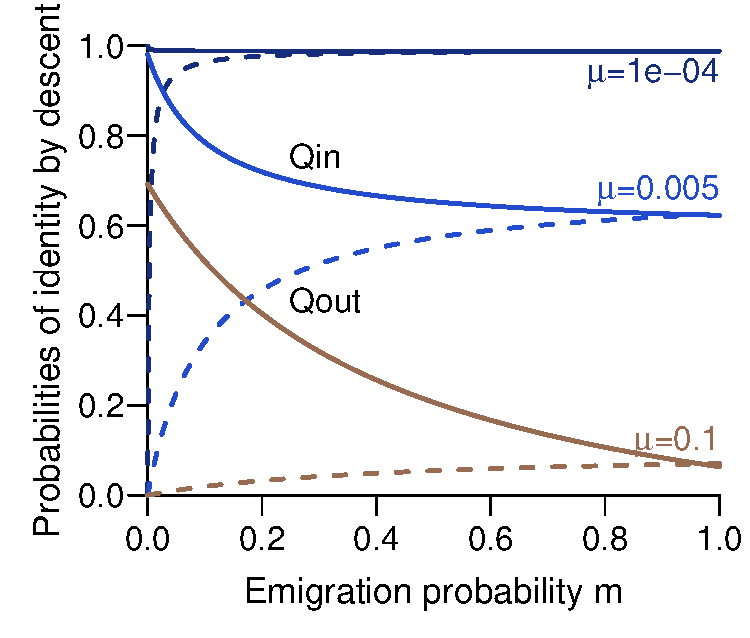
\includegraphics[width = \wpic]{../Programs/R/Pics/QplotM.pdf}}
&
\subfigure[\label{fig:sub:QWF}Wight-Fisher]{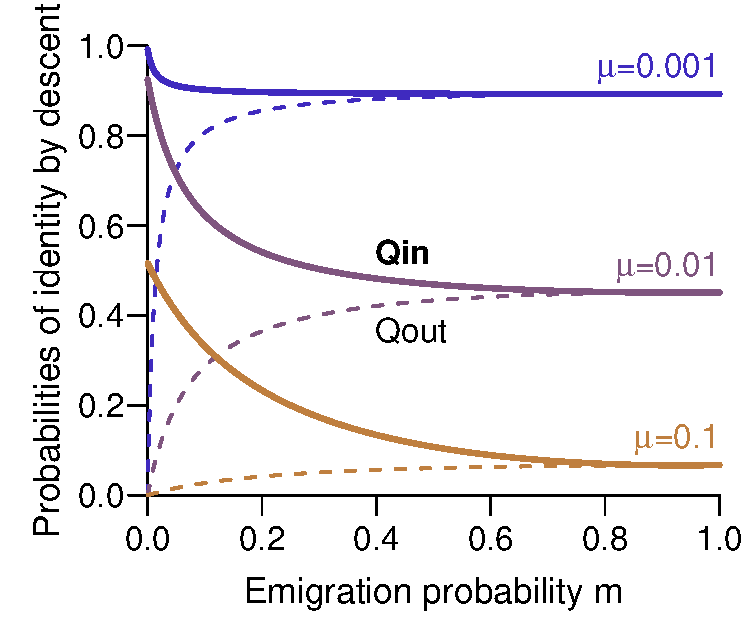
\includegraphics[width = \wpic]{../Programs/R/Pics/QplotWF.pdf}}
\end{tabular}
\caption{Probabilities of identity by descent, for two different individuals within the same deme ($\Qin$, full curves) and two individuals in different demes ($\Qout$, dashed curves), for different values of the mutation probability $\mu$ ($10^{-4}$, $0.005$, $0.1$), and for the two types of life-cycles: Moran \subref{fig:sub:QM} and Wright-Fisher \subref{fig:sub:QWF}. Other parameters: $n=4$ individuals per deme, $\ndemes = 30$ demes. }
\label{fig:Q}
\end{figure}


\subsection{Expected frequencies of altruists for each life-cycle}

For each of the life-cycles that we consider, we can express $\deriv{\Esp{\overline{X}}}{\omega}$ as follows:
\begin{equation}\label{eq:dEXgeneric}
\deriv{\Esp{\overline{X}}}{\omega} = \frac{p (1-p)}{\mu} \left[ \bb \left( \beta_{\direct} - \beta_{\indirect} \right) - \cc \left( \gamma_{\direct} - \gamma_{\indirect} \right) \right],
\end{equation} 
where the subscript $_{\direct}$ refers to ``direct'' effects, and the subscript $_{\indirect}$ to ``indirect'' effects. These indirect effects correspond to (kin) competition: by providing a benefit to a deme-mate and thereby increasing its fecundity, a focal altruist indirectly harms others by reducing their relative fecundity. Similarly, paying a fecundity cost indirectly helps others because it increases their relative fecundities. 

\subsubsection{Direct effects}
Direct effects are similar for the three life-cycles; the only difference is the value of probabilities of identity by descent $Q$, that differ between Moran and Wright-Fisher life-cycles, as seen in the previous section:
%
\begin{subequations}\label{eq:directeffects}
\begin{align}
\beta_{\direct}^{\BD} = \beta_{\direct}^{\DB} &= \left( 1-\mu\right) \Qin^{\Moran}, \label{eq:bBDD}\\
\beta_{\direct}^{\WF} &= \left( 1-\mu\right) \Qin^{\WF}; \label{eq:bWFD}\\
%
%
\gamma_{\direct}^{\BD} = \gamma_{\direct}^{\BD} = \gamma_{\direct}^{\WF} &= 1-\mu.\label{eq:cBDD}
\end{align}
\end{subequations}
%
For both benefits and costs, direct effects only count when there is no mutation ($1-\mu$). Direct effects of benefits ($\bb$) only count if the interaction takes place with an individual who is identical by descent; interactions occurs only within demes, hence the presence of $\Qin$ in \eqref{eq:bBDD} and \eqref{eq:bWFD}. The direct effect of the fecundity cost $\cc$ however does not depend on the type of interactant. 

As seen in the previous section, $\Qin^{\Moran}$ and $\Qin^{\WF}$ decrease with the emigration probability $m$ (actually only until $m=\frac{d-1}{d}$ for the latter). Consequently, the magnitude of the direct (beneficial) effects of benefits $\bb$ provided by altruists ($\beta_{\direct}$) decreases, while the direct (costly) effects ($\gamma_{\direct}$) due to the direct cost of altruism $\cc$ are constant. As a result, if we only consider direct effects, more emigration $m$ is detrimental to the evolution of altruistic behaviour. But there are also indirect effects at play. 

\subsubsection{Indirect effects}
Indirect effects are collateral effects on other individuals; they depend on the type of life-cycle, but always involve individuals who are identical by descent. 

\paragraph{Moran Birth-Death} Changing the fecundity of a focal individual has two types of indirect effects on others: \begin{inparaenum}[\it i\rm )]\item it affects their probability of being the one chosen to reproduce -- this affects all individuals in the population who are identical by descent to the focal, and \item it affects their probability of dying because the number of offspring landing in their site changes -- this affects individuals in the population who can send offspring at the same locations as the focal and are identical-by-descent to it; we obtain  \end{inparaenum}
%
\begin{subequations}
\begin{equation}\label{eq:bBDI}
\begin{split}
\beta_{\indirect}^{\BD} &=  (1-m) \left(\frac{n-1}{n} \Qin^{\Moran} + \frac{1}{n}\right) + m \, \Qout^{\Moran} %
- \mu \frac{ 1 + (n-1) \Qin^{\Moran} + n (d-1) \Qout^{\Moran}}{n d} \\
&= \gamma_{\direct}^{\BD}.
\end{split}
\end{equation}
%
The formulas are the same for the indirect effects associated to $\bb$ and to $\cc$; in other words, the balance between the two indirect effects remains the same when the emigration probability changes. The term $\left(\frac{n-1}{n} \Qin^{\Moran} + \frac{1}{n}\right)$, which we will see appear again later, corresponds to the probability that two individuals sampled with replacement from the same deme are identical by descent. Indirect effects are indeed also felt by the focal individual itself (\eg, increasing the fecundity of another individual implies decreasing one's own relative fecundity). 

Replacing $\Qin$ and $\Qout$ by their formula for the Moran life-cycle (\eqref{eq:QM}), we see that both are decreasing functions of the emigration probability $m$.

\subsubsection{Moran Death-Birth} With this life-cycle,  death comes first and every individual in the population has the same survival probability ($1/N$). The indirect consequences of changing a focal individual's fecundity affect all individuals who can send their offspring to the same locations are the focal, and are identical by descent to it. We obtain
\begin{equation}\label{eq:bDBI}
\begin{split}
\beta_{\indirect}^{\DB} & = (1-\mu ) \Bigg[ \left( \frac{1}{n} + \frac{ (n-1) \Qin^{\Moran} }{n} \right) \left( (1-m)^2 +  \frac{m^2}{ (d-1)} \right) \\ 
%
& \qquad \qquad \quad + m \, \left(2  (1-m) +  (d-2) \frac{m}{(d-1)}\right) \Qout^{\Moran} \Bigg] \\
& = \gamma_{\indirect}^{\DB}
%
\end{split}
\end{equation}
The first term within the brackets in \eqref{eq:bDBI} corresponds individuals from the same deme whose offspring either does not emigrate, or emigrate to the same deme, and the second term, to individuals from different demes who end up in the same location (either one of their demes, or a third deme). 

Here again, $\beta_{\indirect}=\gamma_{\indirect}$, so the balance between the two does not change when the emigration probability $m$ increases.

Replacing $\Qin$ and $\Qout$ by their formulas given in \eqref{eq:QM}, we can see that  $\beta_{\indirect}=\gamma_{\indirect}$ first decreases with the emigration probability $m$, and increases again after a threshold value $m_c'$ (given in the appendix; $m_c' < (d-1)/d$)\todo{name}.  

\subsubsection{Wright-Fisher} Generations are synchronous, and all individuals again all have the same survival probability (now equal to $0$). As a result, the formulas for $\beta_{\indirect}^{\WF}$ and $\gamma_{\indirect}^{\WF}$ are the same as $\beta_{\indirect}^{\DB}$ and $\gamma_{\indirect}^{\WF}$, except that instead of $\Qin^{\Moran}$ and $\Qout^{\Moran}$, we need to use $\Qin^{\WF}$ and $\Qout^{\WF}$ (given in \eqref{eq:QWF}). Once this is done, we see that $\beta_{\indirect}^{\WF} = \gamma_{\indirect}^{\WF} =$ first decreases with the emigration probability $m$, and increases again after the threshold value $m_c = (d-1)/d$ (which was identified previously as the emigration probability such that offspring have an equal chance of landing in their natal deme or in any other deme). 
\end{subequations}

\subsection{Identifying threshold values of the mutation probability $\mu$}

In the previous section, we investigated the impact of changes in the emigration probability $m$ on each of the terms that make up the expected frequency of altruists $\Esp{\overline{X}}$. Now we need to combine these different terms to focus on the quantity we are eventually interested in, $\Esp{\overline{X}}$. The rather lengthy formulas that we obtain are relegated to the \hl{appendix}, and we concentrate here on the results. 

\subsubsection{Moran Birth-Death}

For this life-cycle, we find that the expected frequency of altruists $\Esp{\overline{X}}$ is a monotonic function of the emigration probability $m$; the direction of the change depends on the value of the mutation probability $\mu$ compared to a threshold value $\mu_c^{\BD}$. When $\mu<\mu_c^{\BD}$, $\Esp{\overline{X}}$ decreases with $m$, while when $\mu>\mu_c^{\BD}$, $\Esp{\overline{X}}$  increases with $m$; $\mu_c^{\BD}$ is given by 
\begin{equation}\label{eq:mucBD}
\mu_c^{\BD} = %
1 - \frac{\bb  - \cc + \sqrt{(\bb - \cc) \left(4 \bb (n d)^2 + \bb - \cc \right)} }{2 \bb n d}
\end{equation}
%
This result is illustrated in figure~\ref{fig:EX}\subref{fig:EXBD}\todo{donner la valeur}.


\subsubsection{Moran Death-Birth}

The relationship between $\Esp{\overline{X}}$ and $m$ is a bit more complicated for this life-cycle. For simplicity, we concentrate on what happens starting from low emigration probabilities. If the benefits $\bb$ provided by altruists are relatively low ($\bb < \cc (n+1)$), $\Esp{\overline{X}}$ initially increases with $m$ provided the mutation probability $\mu$ is greater than a threshold value $\mu_c^{\DB}$ given in \eqref{eq:mucDB} below; otherwise, when the benefits are high enough, $\Esp{\overline{X}}$ initially increases with $m$ for any value of $\mu$. Combining these results, we write
\begin{equation}\label{eq:mucDB}
\mu_c^{\DB} = \begin{cases}
\dfrac{\bb -  (n+1) \cc}{ (n-1) \cc - (2 n - 1) \bb} & \textrm{if $\bb < \cc (n+1)$,} \\
%
0 & \textrm{otherwise. }
\end{cases}
\end{equation} 
The expected frequency of altruists $\Esp{\overline{X}}$ reaches a maximum for an emigration probability $m_c^{\DB}$ (whose complicated\todo{do} equation is in the \hl{appendix}), as can be seen in figure~\ref{fig:EX}\subref{fig:EXDB}. The limit of this critical emigration probability $m_c^{\DB}$ when $\mu \to 0$ is $0$\todo{attention order of limits}: we recover the result that more emigration is detrimental to the evolution of altruism when the mutation probability is either null or vanishingly small. \todo{appendix}

\subsubsection{Wright-Fisher}

The expected frequency of altruists in the population reaches an extremum when $m = m_c^{\WF} = \frac{d-1}{d}$. This extremum is a maximum when the mutation probability is higher than a threshold value $\mu_c^{\WF}$ given by 
\begin{equation}
\mu_c^{\WF} = 1-\sqrt{1-\frac{\cc}{\bb}},
\end{equation}
and it is a minimum otherwise (see figure~\ref{fig:EX}\subref{fig:EXWF}). 

% Figure weak selection
\begin{figure}
\begin{tabular}{ccc}
\subfigure[Death-Birth \label{fig:EXDB}]{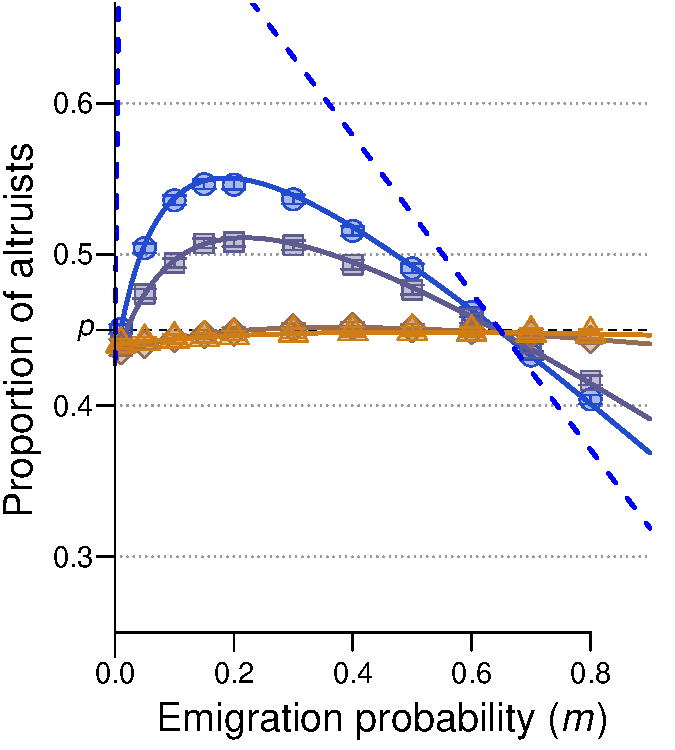
\includegraphics[type=pdf,ext=.pdf,read=.pdf, width=5cm]{../Programs/R/Pics/EXDB_sel0.005_htg0}}
&
\subfigure[Birth-Death \label{fig:EXBD}]{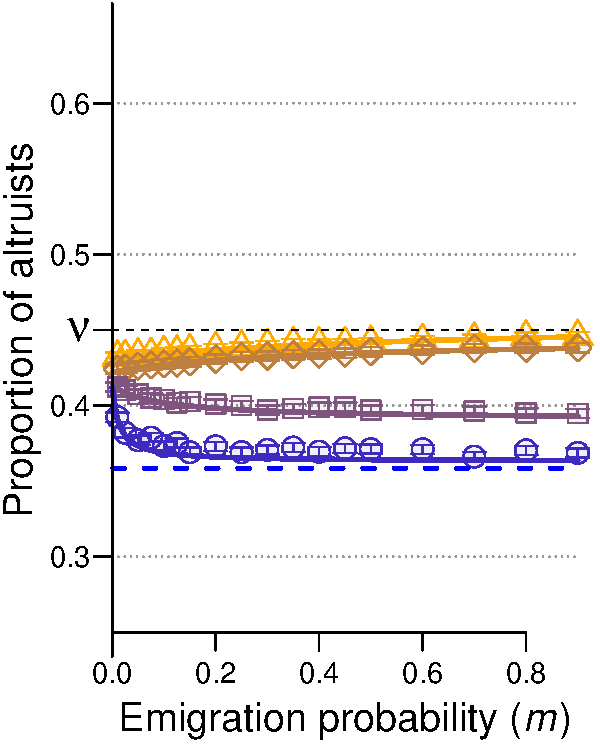
\includegraphics[type=pdf,ext=.pdf,read=.pdf, width=5cm]{../Programs/R/Pics/EXBD_sel0.005_htg0}}
&
\subfigure[Wright-Fisher \label{fig:EXWF}]{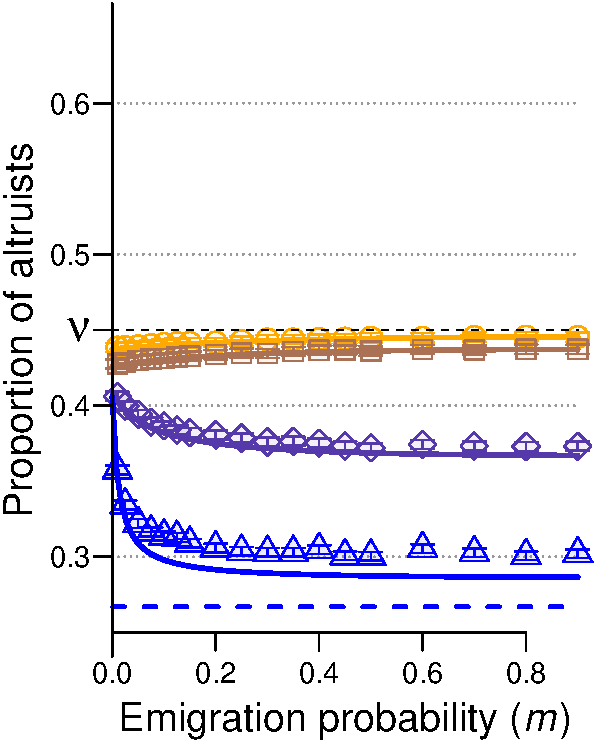
\includegraphics[type=pdf,ext=.pdf,read=.pdf, width=5cm]{../Programs/R/Pics/EXWF_sel0.005_htg0}}
\end{tabular}
\caption{Weak selection. Parameters: $\omega = 0.005$, $b = 15$, $c = 1$, \hl{ndemes, size, nreps}. NOTE simulations running with 0.005 for mu and with 0.8 for mig. }
\label{fig:EX}
\end{figure}

\subsection{Relaxing key assumptions}

To derive our analytical results, we had to make a number of simplifying assumptions, such as the fact that selection is weak ($\omega \ll 1$), and the fact that the structure of the population is regular (all demes have the same size $n$). We explored with numerical simulations the effect of relaxing these key assumptions. The patterns that we identified hold when selection is strong (see figure~\ref{fig:EXstrongsel}, done with $\omega = 0.1$), but also when the demes have different sizes. Deme sizes are drawn randomly at the beginning of a simulation; the range from $1$ to $5$ individuals per deme and the average size is $4$ individuals as in the other figures.\todo{le pb c'est ptet simplement que 1 individu ca pose probleme!}. Here as well, the same patterns hold as those obtained with a homogeneous structure (figure~\ref{fig:EXhtg}). Add\todo{todo} effect of $\dself$.

\section{Discussion}

% Summary
Adding non zero mutation probability altruism increases with emigration. 

% Measure of altruism
Quantitative measure of the success of altruism: $\Esp{\overline{X}}$. Qualitative measure commonly used is whether greater than $p$: no effect on BD and WF, but still effect on DB. 

% How to explain the result
Go back to the decomposition of the different terms, we see that increase of $\Esp{\overline{X}}$ with $m$ is driven by the $\beta_{\indirect}$ term. To simplify the explanations, let us consider that the number of demes is large: in this case, $\Qout$ is vanishingly small and so terms involving it can be omitted. Let us also assume that there is no direct cost to being an altruist ($\cc = 0$). 

% Order of limits
Problems of orders of limits, especially when $d \to \infty$ and $\mu \to 0$. Need to specify how small the mutation probability is compared to the size of the population. 

% Steve Frank
Difference with Steve Frank: $R$ was a model parameter, \ie, the same for different emigration probabilities. 

% Links votant
Voter model


%%% ___ BIBLIO _____
\clearpage
\bibliographystyle{amnat}

\bibliography{bibSCSP}

\clearpage
% Start the appendix
\appendix
 
% Redefine counters
% Equations
%  Redefine the command that creates the equation number.
\renewcommand{\theequation}{\thesection.\arabic{equation}}
%  Reset the counter
\setcounter{equation}{0}  % reset counter
 
% Figures
%  Redefine the command that creates the figure number: adds an S.
\renewcommand{\thefigure}{S\arabic{figure}}
%  Reset the counter  
\setcounter{figure}{0}

\section*{Supplementary figures} 

% Figure strong selection
\begin{figure}[h!]
\begin{tabular}{ccc}
\subfigure[Death-Birth]{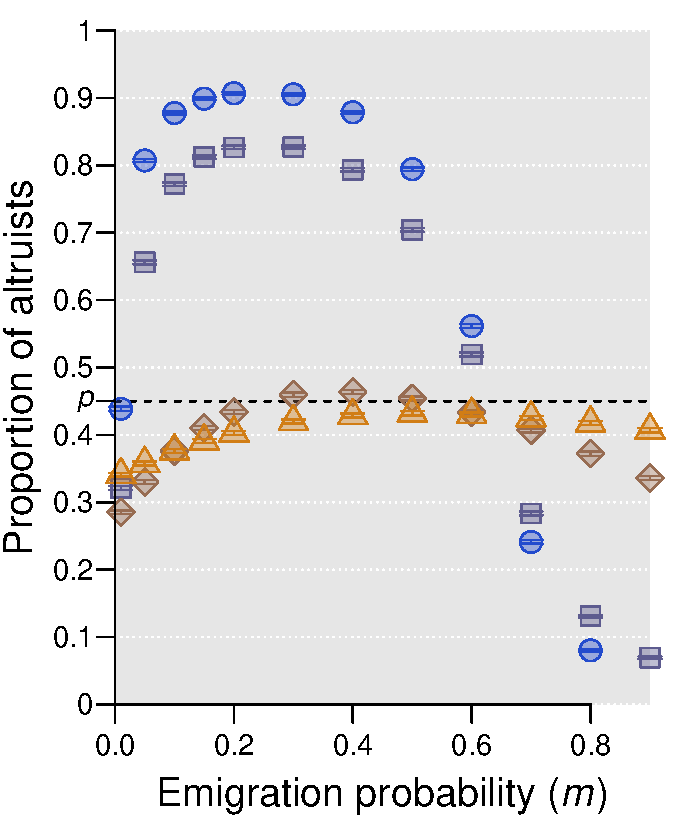
\includegraphics[type=pdf,ext=.pdf,read=.pdf, width=5cm]{../Programs/R/Pics/EXDB_sel0.1_htg0}}
&
\subfigure[Birth-Death]{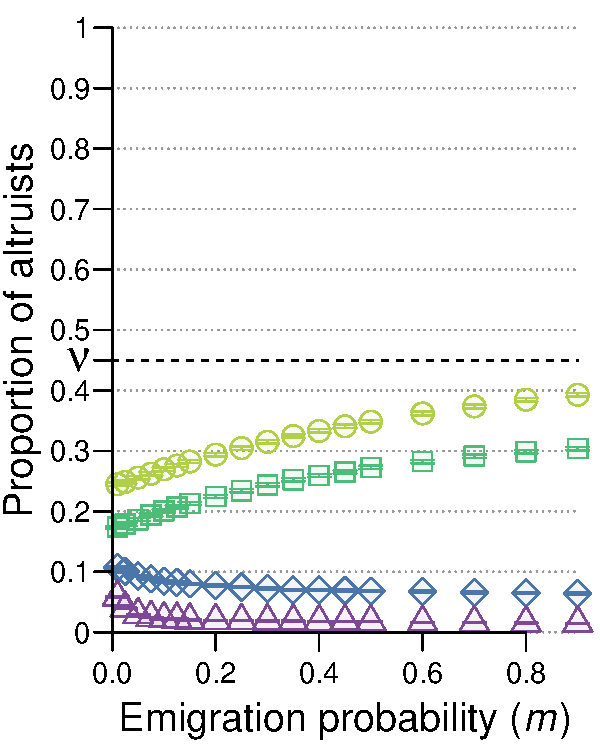
\includegraphics[type=pdf,ext=.pdf,read=.pdf, width=5cm]{../Programs/R/Pics/EXBD_sel0.1_htg0}}
&
\subfigure[Wright-Fisher]{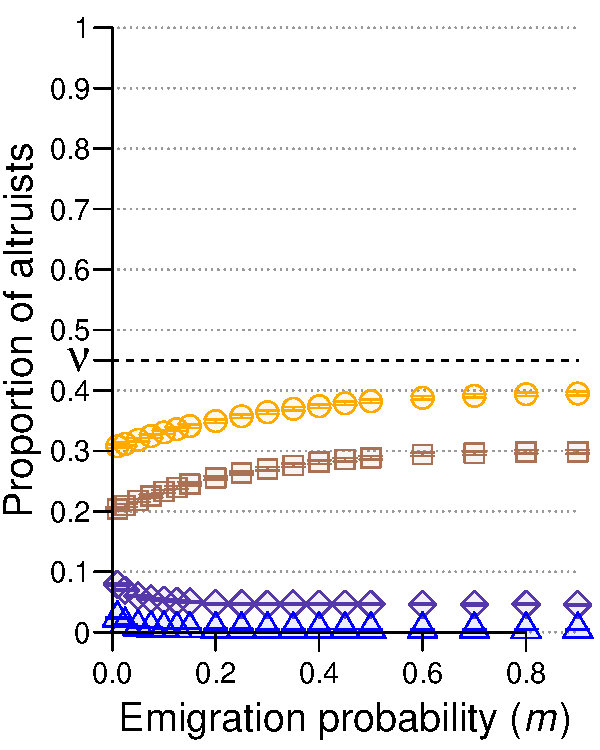
\includegraphics[type=pdf,ext=.pdf,read=.pdf, width=5cm]{../Programs/R/Pics/EXWF_sel0.1_htg0}}
\end{tabular}
\caption{Equivalent of figure~\ref{fig:EX} but with strong selection ($\omega = 0.1$); all other parameters and legend are identical to those of figure~\ref{fig:EX}. }
\label{fig:ESstrongsel}
\end{figure}

% Figure heterogeneous population
\begin{figure}
\begin{tabular}{ccc}
\subfigure[Death-Birth]{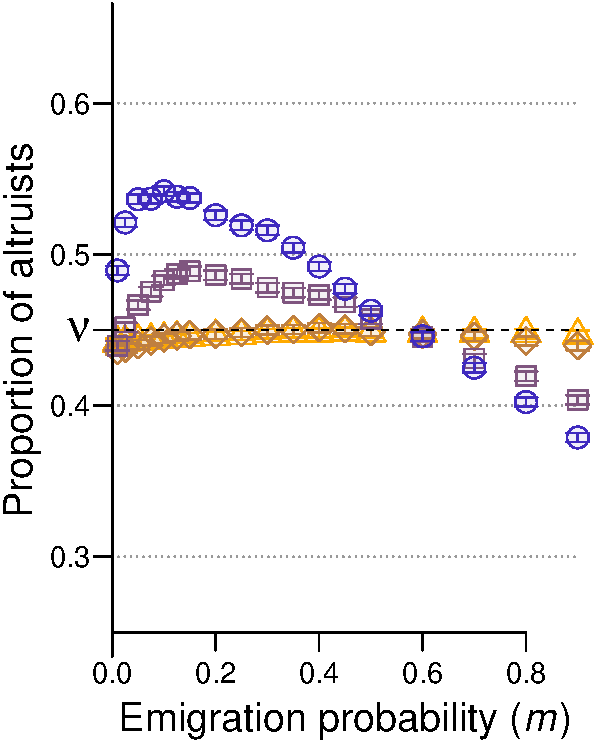
\includegraphics[type=pdf,ext=.pdf,read=.pdf, width=5cm]{../Programs/R/Pics/EXDB_sel0.005_htg1}}
&
\subfigure[Birth-Death]{
\includegraphics[type=pdf,ext=.pdf,read=.pdf, width=5cm]{../Programs/R/Pics/EXBD_sel0.005_htg1}}
&
\subfigure[Wright-Fisher]{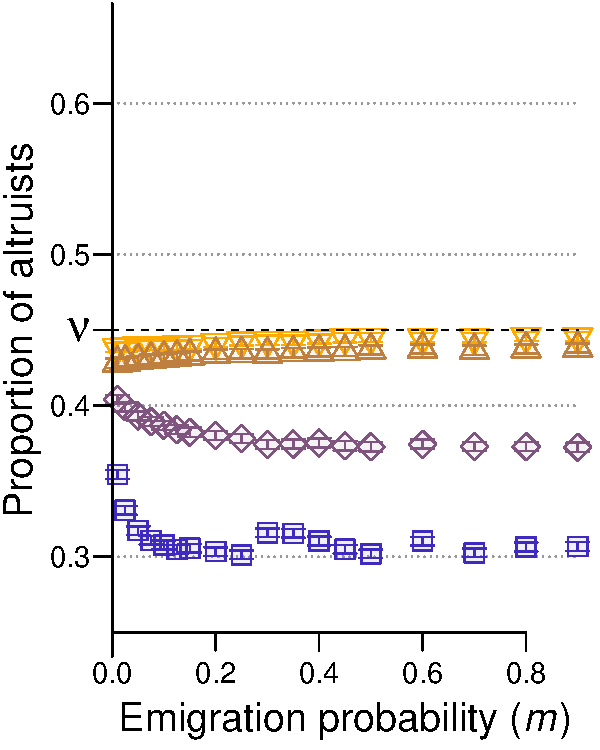
\includegraphics[type=pdf,ext=.pdf,read=.pdf, width=5cm]{../Programs/R/Pics/EXWF_sel0.005_htg1}}\end{tabular}
\caption{Equivalent of figure~\ref{fig:EX} but with a heterogeneous population structure: deme sizes range form $1$ to $5$ individuals per deme, the average deme size is $4$ as in figure~\ref{fig:EX};  all other parameters and legend are identical to those of figure~\ref{fig:EX}. }
\label{fig:EXhtg}
\end{figure}


 
\clearpage
% Figure heterogeneous population
\begin{figure}
\begin{tabular}{ccc}
\subfigure[Death-Birth]{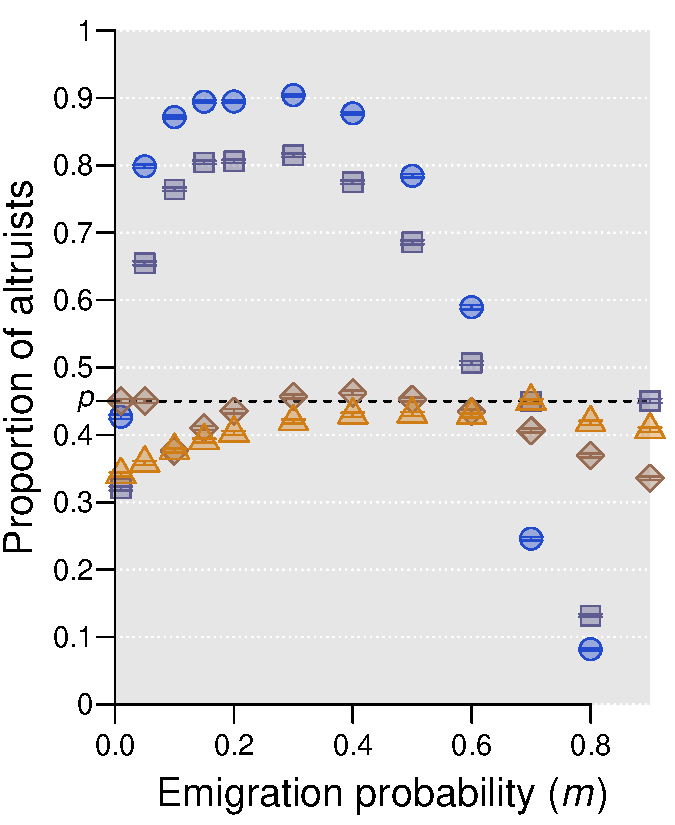
\includegraphics[type=pdf,ext=.pdf,read=.pdf, width=5cm]{../Programs/R/Pics/EXDB_sel0.1_htg1}}
&
\subfigure[Birth-Death]{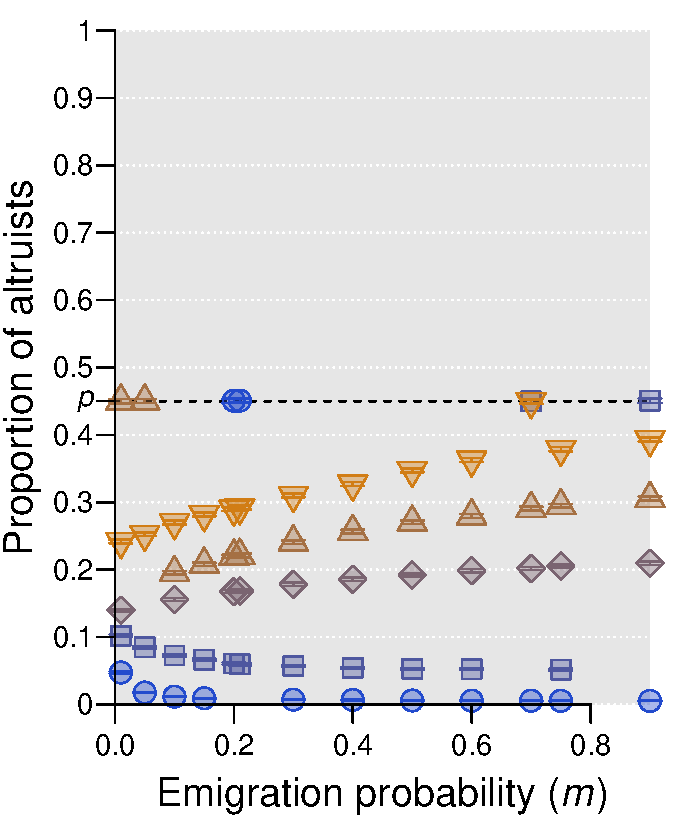
\includegraphics[type=pdf,ext=.pdf,read=.pdf, width=5cm]{../Programs/R/Pics/EXBD_sel0.1_htg1}}
&
\subfigure[Wright-Fisher]{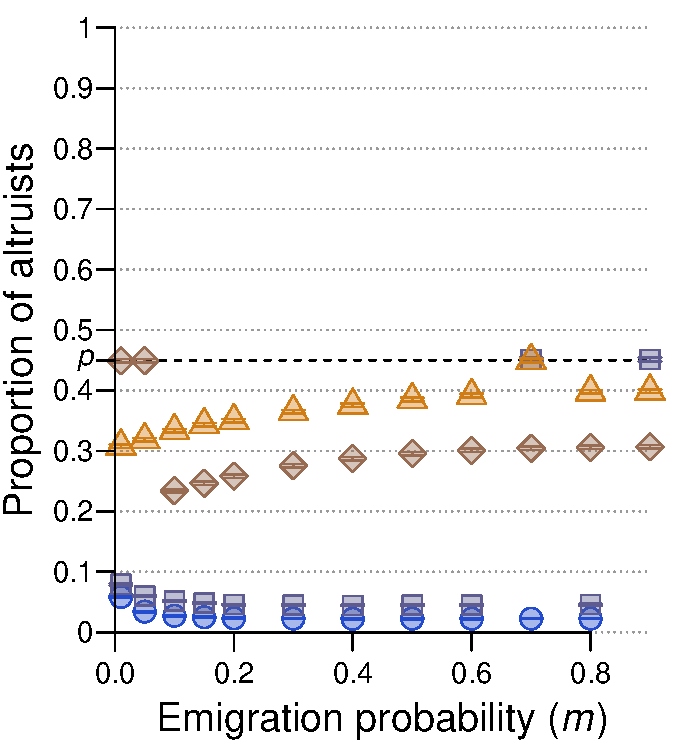
\includegraphics[type=pdf,ext=.pdf,read=.pdf, width=5cm]{../Programs/R/Pics/EXWF_sel0.1_htg1}}\end{tabular}
\caption{Strong selection, heterogeneous population}
\label{fig:island_htgpop}
\end{figure}

\clearpage
Adaptation of my equations to a subdivided population. Notation, for a quantity $Y$ that depends on two sites ($Y=e$, $d$, $Q$):
\begin{subequations}
\begin{align}
Y_{\textrm{self}} &\defeq Y_{i,i} \\
%
Y_{\textrm{in}} &\defeq Y_{i,j}, \quad \textrm{$i$ and $j\neq i$ in the same deme;}\\
%
Y_{\textrm{out}} &\defeq Y_{i,j}, \quad \textrm{$i$ and $j$ in different demes.}
\end{align}
\end{subequations}
For a site $i$, $G_i$ denotes the deme the site belongs to, and notation $j \in G_i$ means that sites $i$ and $j$ are in the same deme. 

The expected frequency of altruists in the population is given by 
\begin{equation}
\Esp{\overline{X}} = p + \delta \frac{p (1-p)}{\mu} \left[ \bb \, (\beta^{D} - \beta^{I}) - \cc \, (\gamma^{D} - \gamma^{I}) \right].
\end{equation}

\paragraph{Moran, Birth-Death}

\begin{subequations}
\begin{align}
\beta_{\BD}^{D} =& \sum_{k,\ell = 1}^N \frac{1-\mu}{N} e_{kl} Q_{lk} \nonumber \\
%
= & \sum_{k=1}^N \frac{1-\mu}{N} \Big( \eself + (n-1) \ein \Qin + (N-n) \eout \Qout \Big) \nonumber \\
%
= & (1-\mu) \Big( \eself + (n-1) \ein \Qin + (N-n) \eout \Qout \Big).
\end{align}

\begin{align}
\beta_{\BD}^{I} =& \sum_{j,k,l=1}^N \left( \frac{d_{lj}}{N} - \frac{\mu}{N^2}\right) e_{kl} Q_{jk} \nonumber \\
%
= & \frac{1}{N}\sum_{j=1}^N \Bigg[ \left( \sum_{l=1}^N  d_{lj}  e_{jl}  \right)%
+ \sum_{\substack{k \in G_j \\ k\neq j}} \left( \sum_{l=1}^N d_{lj}  e_{kl} \Qin  \Qin \right)%
%\nonumber \\&
+ \sum_{k \not\in G_j}\sum_{l=1}^N d_{lj}  \left( e_{kl} \Qout  \Qout \right)\Bigg] \nonumber \\
& + \frac{\mu}{N^2} \sum_{j=1}^N \left( \sum_{l=1}^N e_{kl} \right) \left( \sum_{k=1}^N Q_{jk} \right) \nonumber \\
%
= & \frac{1}{N} \sum_{j=1}^N\Bigg[ \dself \eself + (n-1) \din \ein + (N-n) \dout \eout \nonumber\\
& \quad + \sum_{\substack{k \in G_j \\ k\neq j}} \left( \din  \eself + \dself  \ein + (n-2) \din \ein + (N-n) \dout  \eout  \right) \Qin \nonumber\\
& \quad + \sum_{k \not \in G_j} \left( \dself  \eout + (n-1) \din  \eout + \dout \eself + (n-1) \dout \ein + (N - 2n) \dout \eout \right) \Qout \nonumber \Bigg] \\
& - \frac{\mu}{N} \left(1 + (n-1)\Qin + (N-n) \Qout\right) \left( \eself + (n-1) \ein + (N-n)\eout \right) \nonumber \\
%
%
= & \dself \eself + (n-1) \din \ein + (N-n) \dout \eout \nonumber\\
& + (n-1) \left( \din  \eself + \dself  \ein + (n-2) \din \ein + (N-n) \dout  \eout  \right) \Qin \nonumber\\
& + (N-n) \left( \dself  \eout + (n-1) \din  \eout + \dout \eself + (n-1) \dout \ein + (N - 2n) \dout \eout \right) \Qout \nonumber  \\
& - \frac{\mu}{N} \left(1 + (n-1)\Qin + (N-n) \Qout\right) \left( \eself + (n-1) \ein + (N-n)\eout \right).
\end{align}

\begin{align}
\gamma_{\BD}^{D} & = 1-\mu.
\end{align}

\begin{align}
\gamma_{\BD}^{I} & = \frac{1}{N} \sum_{j,k=1}^N \left( d_{kj} - \frac{\mu}{N}  \right) Q_{jk}\nonumber \\
& = \frac{1}{N} \sum_{j=1}^N \left[ \dself - \frac{\mu}{N} + (n-1) \left( \din - \frac{\mu}{N} \right) \Qin + (N-n) \left( \dout - \frac{\mu}{N} \right) \Qout\right] \nonumber \\
%
& = \dself + (n-1) \din\Qin + (N-n)\dout \Qout \nonumber \\&\quad - \frac{\mu}{N} \left(1 + (n-1)\Qin + (N-n) \Qout\right)
\end{align}
\end{subequations}

\paragraph{Moran, Death-Birth}
\begin{subequations}
\begin{align}
\beta_{\DB}^{D} & = \frac{1-\mu}{N} \sum_{j,k=1}^N Q_{jk} e_{jk} = \beta_{\BD}^D\nonumber \\
& = (1-\mu) \Big( \eself + (n-1) \ein \Qin + (N-n) \eout \Qout \Big).
\end{align}

\begin{align}
\beta_{\DB}^{I} & = \frac{1-\mu}{N} \sum_{i,j,k,l=1}^N d_{ji} d_{li} e_{kl} Q_{jk} 
\end{align}
Presented in the table in the appendix.

\begin{align}
\gamma_{\DB}^{D} & = 1-\mu = \gamma_{\BD}^{D}.
\end{align}

\begin{align}
\gamma_{\DB}^{I} & = (1-\mu) \sum_{i,j,k=1}^N \frac{d_{ji} d_{ki}}{N} Q_{jk} \nonumber \\
%
& = \frac{1-\mu}{N} \sum_{j=1}^N \sum_{i=1}^N \Big( d_{ji} d_{ji} + \sum_{\substack{k\neq j\\ k \in G_j}} d_{ji} d_{ki} \Qin + \sum_{k \not \in G_j} d_{ji} d_{ki} \Qout \Big) \nonumber \\
%
& = \frac{1-\mu}{N} \sum_{j=1}^N \Bigg[ \dself \dself + (n-1) \din \din + (N-n) \dout \dout \nonumber \\
%
& \qquad +(n-1) \Big( \dself \din + \din \dself + (n-2) \din \din + (N-n) \dout \dout \Big) \Qin \nonumber \\
%
& \qquad + (N-n)\Big( \dself \dout + (n-1)\din \dout + \dout \dself + (n-1)\dout \din + (N-2n) \dout \dout
\Big)\Qout
\Bigg]
\end{align}

\end{subequations}

\subsection*{Probabilities of identity by descent}
\hl{WF est faux. Il faut utiliser les formules Fourier...!}
\paragraph{Moran}
\begin{subequations}
For $i=\neq j$,
\begin{align}
Q_{ij} = \frac{1-\mu}{2} \sum_{k=1}^N \left( d_{kj} Q_{ki} + d_{ki} Q_{kj} \right).
\end{align}
For $j\neq i$, $j\in G_i$, 
\begin{align}
\Qin & = \frac{1-\mu}{2} \Big( \left( \din + \dself \Qin \right)  + \left( \dself \Qin + \din \right) \nonumber \\ 
& \qquad  + (n-2) \left( \din \Qin + \din \Qin \right) + (N-n) \left( \dout \Qout  + \dout \Qout  \right)  \Big) \nonumber \\
% 
& = (1-\mu) \Big( \din + \dself \Qin + (n-2) \din \Qin + (N-n) \dout \Qout  \Big).
\end{align}
And for $j \not \in G_i$, 
\begin{align}
\Qout & = \frac{1-\mu}{2} \Big( \left( \dout  + \dself \Qout \right) + (n-1) \left( \dout \Qin + \din \Qout \right) \nonumber\\
& \qquad + \left( \dself \Qout + \dout \right) + (n-1) \left( \din \Qout + \dout \Qin \right) \nonumber \\
& \qquad + (N-2n)\left( \dout \Qout + \dout \Qout \right)\Big) \nonumber \\
%
& = (1-\mu) \Big(  \dout  + \dself \Qout  + (n-1) \left( \dout \Qin + \din \Qout \right) + (N-2n) \dout \Qout \Big)
\end{align}
\end{subequations}

\paragraph{Wright-Fisher}

\begin{subequations}
For $j\neq i$,
\begin{align}
Q_{ij} &= (1-\mu)^2 \sum_{k,l=1}^N d_{ki} d_{lj} Q_{kl}.
\end{align}
When $j\neq i$, $j\in G_i$, 
\begin{align}
\Qin & = (1-\mu)^2 \Bigg[ \Big( \dself \din + \din \dself + (n-2) \din \din + (N-n) \dout \dout \Big)\nonumber\\
%
& \qquad + \Big( \dself \dself + (n-2) \dself \din \nonumber\\ & \qquad \qquad + (n-1) \din \din + (n-2) \din \dself \nonumber\\
& \qquad\qquad+ (n-2)(n-2) \din \din + (N-n) (n-1)\dout \dout  \Big) \Qin \nonumber \\
%
& \qquad + \Big((N-n) \dself \dout + (N-n)(n-1) \din \dout \nonumber \\ 
& \qquad\qquad+ (N-n) \dout \dself + (N-n)(n-1) \dout \din \nonumber \\ 
& \qquad\qquad+ (N-n)(N-2n) \dout \dout \Big) \Qout \Bigg]\nonumber\\
%
%
%
& = (1-\mu)^2 \Bigg[ \Big( 2 \din \dself + (n-2) \din^2 + (N-n) \dout^2 \Big) \nonumber\\
&\qquad + \Big( \dself^2 + 2(n-2) \dself \din + (n^2 -3 n +3) \din^2 + + (N-n) (n-1)\dout^2 \Big)\Qin \nonumber \\
& \qquad + \Big(2(N-n) \dself \dout + 2 (N-n)(n-1) \din \dout \nonumber \\ 
& \qquad\qquad+ (N-n)(N-2n) \dout \dout \Big)\Qout
 \Bigg]
\end{align}
And when $j\not \in G_i$, we have
% 
\begin{align}
\Qout & = (1-\mu)^2 \Bigg[ \Big( 2\dself \dout + 2(n-1) \din \dout + (N-2n) \dout^2 \Big)\nonumber \\
& \qquad + \Big( 2(n-1) \dself \dout + 2(n-1)^2 \din \dout + (N-2n)(n-1) \dout^2  \Big)\Qin \nonumber \\
& \qquad +\Big( \dself \dself + (n-1)\dself \din + (N-2n)\dself \dout \nonumber\\
& \qquad \qquad+ (n-1) \din \dself + (n-1)^2 \din^2 + (n-1)(N-2n)\din \dout \nonumber \\
& \qquad \qquad+ (N-n) \dout \dself + (N-n)(n-1) \dout \din + (N-n)(N-2n) \dout \dout \Big) \Qout \Bigg].
\end{align}
\hl{PAS FINI}
\end{subequations}
\clearpage
\appendix
\section*{Appendix}
All combinations for $i$, $j$, $k$, $l$. Notation: $(i, j)$ means that $i$ and $j$ are in the same deme, but are different; $G_i$ refers to the deme containing site $i$.

\begin{landscape}

\rowcolors{2}{gray!25}{white}
\begin{longtable}{>{\footnotesize $}l<{$} >{\small $}l<{$} >{\small $}l<{$} >{\small $}l<{$}   >{$}l<{$}   >{$}l<{$}   >{$}l<{$}   >{$}l<{$}  >{$}l<{$} >{$}l<{$} }
\rowcolor{gray!60}
%\hline
& j & k & l & \textrm{Notation} & \textrm{Count}  & d_{ji} & d_{li} & e_{kl} & Q_{jk} \\
%\hline
\endhead % all the lines above this will be repeated on every page
%
1 & j=i & k=i & l = i & (i = j= k =l) & 1 & \dself & \dself & \eself & 1 \\*
%
2 & j=i & k=i & l\neq i; l \in G_i & (i=j=k, l) & n-1 & \dself & \din & \ein & 1\\*
%
3 & j=i & k=i & l\not \in G_i & (i=j=k), (l) & N-n & \dself & \dout & \eout & 1 \\
%
%
4 & j=i & k\neq i; k\in G_i & l=i & (i=j=l, k) & n-1 & \dself & \dself & \ein & \Qin \\*
%
5 & j=i & k\neq i; k\in G_i & l=k & (i=j, k=l) & n-1 & \dself & \din & \eself & \Qin \\*
%
6 & j=i & k\neq i; k\in G_i & l\neq i, k; l\in G_i & (i=j, k, l) & (n-1)(n-2) & \dself & \din & \ein & \Qin \\*
%
7 & j=i & k\neq i; k\in G_i & l\not \in G_i & (i=j, k), (l) & (n-1)(N-n) & \dself &  \dout & \eout & \Qin \\
%
%
8 & j=i & k\not \in G_i & l=i=j & (i=j=l), (k) & (N-n) & \dself & \dself & \eout & \Qout \\*
%
9 & j=i & k\not \in G_i & l\neq i, l\in G_i & (i=j, l), (k) & (N-n)(n-1) & \dself & \din & \eout & \Qout \\*
%
10 & j=i & k\not \in G_i & l=k & (i=j), (k=l) & (N-n) & \dself & \dout & \eself & \Qout \\*
%
11 & j=i & k\not \in G_i & l\neq k; l\in G_k & (i=j), (k, l) & (N-n)(n-1) & \dself & \dout & \ein & \Qout \\*
%
12 & j=i & k\not \in G_i & l\not \in G_i, G_k & (i=j), (k), (l) & (N-n)(N-2n) & \dself & \dout & \eout & \Qout \\
%
%
%
%
13 & j\neq i, j\in G_i & k=i & l=i & (i=k=l, j) & (n-1) & \din & \dself & \eself & \Qin \\*
%
14 & j\neq i, j\in G_i & k=i & l=j & (i=k, j=l) & (n-1) & \din & \din & \ein & \Qin \\*
%
15 & j\neq i, j\in G_i & k=i & l\neq i, j; l\in G_i & (i=k, j, l) & (n-1)(n-2) & \din & \din & \ein & \Qin \\*
%
16 & j\neq i, j\in G_i & k=i & l\not \in G_i & (i=k, j), (l) & (n-1)(N-n) & \din & \dout & \eout & \Qin \\
%
%
17 & j\neq i, j\in G_i & k=j & l=i & (i=l, j=k) & (n-1) & \din & \dself & \ein & 1 \\*
%
18 & j\neq i, j\in G_i & k=j & l=j & (i, j=k=l) & (n-1) & \din &  \din & \eself & 1\\*
%
19 & j\neq i, j\in G_i & k=j & l\neq i, j; l\in G_i & (i, j=k, l) & (n-1)(n-2) & \din & \din & \ein & 1\\*
%
20 & j\neq i, j\in G_i & k=j & l\not \in G_i & (i, j=k), (l)& (n-1)(N-n) & \din & \dout & \eout & 1\\
%
%
21 & j\neq i, j\in G_i & k\neq i,j; k\in G_i & l=i & (i=l, j, k) & (n-1)(n-2) & \din & \dself & \ein & \Qin \\*
%
22 & j\neq i, j\in G_i & k\neq i,j; k\in G_i & l=j & (i,j=l,k) & (n-1)(n-2) & \din & \din & \ein & \Qin \\*
%
23 & j\neq i, j\in G_i & k\neq i,j; k\in G_i & l=k & (i,j,k=l) & (n-1)(n-2) & \din & \din & \eself & \Qin  \\*
%
24 & j\neq i, j\in G_i & k\neq i,j; k\in G_i & l\neq i,j,k; l
\in G_i & (i,j,k,l) & (n-1)(n-2)(n-3) & \din & \din & \ein & \Qin \\*
%
25 & j\neq i, j\in G_i & k\neq i,j; k\in G_i & l\not \in G_i & (i, j, k), (l) & (n-1)(n-2)(N-n)  & \din & \dout & \eout & \Qin \\
%
%
26 & j\neq i; j\in G_i & k\not\in G_i & l=i & (i=l,j),(k) & (n-1)(N-n) & \din & \dself & \eout & \Qout \\*
%
27 & j\neq i; j\in G_i & k\not\in G_i & l=j & (i, j=l), (k) & (n-1)(N-n) & \din & \din & \eout & \Qout \\*
%
28 & j\neq i; j\in G_i & k\not\in G_i & l\neq i, j; l\in G_i & (i, j, l), (k) & (n-1)(N-n)(n-2) & \din & \din & \eout & \Qout \\*
%
29 & j\neq i; j\in G_i & k\not\in G_i & l=k & (i, j), (k=l) & (n-1)(N-n) & \din & \dout & \eself & \Qout \\*
%
30 & j\neq i; j\in G_i & k\not\in G_i & l\neq k;l\in G_k & (i,j),(k,l) & (n-1)(N-n)(n-1) & \din & \dout & \ein & \Qout \\*
%
31 & j\neq i; j\in G_i & k\not\in G_i & l\not \in G_i, G_k & (i,j),(k),(l) & (n-1)(N-n)(N-2n) & \din & \dout & \eout & \Qout \\
%
%
%
%
32 & j\not\in G_i & k=i & l=i & (i=k=l),(j) & (N-n) & \dout & \dself & \eself & \Qout \\*
%
33 & j\not\in G_i & k=i & l\neq i; l\in G_i & (i=k, l), (j) & (N-n)(n-1) & \dout & \din & \ein & \Qout \\*
%
34 & j\not\in G_i & k=i & l=j & (i=k), (j=l) & (N-n) & \dout & \dout & \eout & \Qout \\*
%
35 & j\not\in G_i & k=i & l\neq j; l\in G_j & (i=k), (j,l) & (N-n)(n-1) & \dout & \dout & \eout & \Qout \\*
%
36 & j\not\in G_i & k=i & l\not \in G_i, G_j & (i=k), (j), (l) & (N-n)(N-2n) & \dout & \dout & \eout & \Qout \\
%
%
37 & j\not\in G_i & k\neq i; k\in G_i & l=i & (i=l, k), (j) & (N-n)(n-1) & \dout & \dself & \ein & \Qout \\*
%
38 & j\not\in G_i & k\neq i; k\in G_i & l=k & (i, k=l), (j) & (N-n)(n-1) & \dout & \din & \eself & \Qout \\*
%
39 & j\not\in G_i & k\neq i; k\in G_i & l\neq i,k; l\in G_i & (i, k, l), (j) & (N-n)(n-1)(n-2) & \dout & \din & \ein & \Qout \\*
%
40 & j\not\in G_i & k\neq i; k\in G_i & l=j & (i, k), (j=l) & (N-n)(n-1) & \dout & \dout & \eout & \Qout \\*
%
41 & j\not\in G_i & k\neq i; k\in G_i & l\neq j;l\in G_j & (i, k), (j,l) & (N-n)(n-1)(n-1) & \dout & \dout & \eout & \Qout \\*
%
42 & j\not\in G_i & k\neq i; k\in G_i & l\not \in G_i,G_j & (i, k), (j),(l) & (N-n)(n-1)(N-2n) & \dout & \dout & \eout & \Qout \\
%
%
43 & j\not\in G_i & k=j & l=i & (i=l), (j=k) & (N-n) & \dout & \dself & \eout & 1 \\*
%
44 & j\not\in G_i & k=j & l\neq i; l\in G_i & (i,l), (j=k) & (N-n)(n-1) & \dout & \din & \eout & 1\\*
%
45 & j\not\in G_i & k=j & l=j & (i), (j=k=l) & (N-n) & \dout & \dout & \eself & 1\\*
%
46 & j\not\in G_i & k=j & l\neq j; l\in G_j & (i), (j=k, l) & (N-n)(n-1) & \dout & \dout & \ein & 1\\*
%
47 & j\not\in G_i & k=j & l\not \in G_i, G_j & (i), (j=k), (l) & (N-n)(N-2n) & \dout & \dout & \eout & 1\\
%
%
48 & j\not\in G_i & k\neq j; k\in G_j & l=i & (i=l), (j, k) & (N-n)(n-1) & \dout & \dself & \eout & \Qin \\*
%
49 & j\not\in G_i & k\neq j; k\in G_j & l\neq i; l\in G_i & (i, l), (j, k) & (N-n)(n-1)(n-1) & \dout & \din & \eout & \Qin\\*
%
50 & j\not\in G_i & k\neq j; k\in G_j & l=j & (i), (j=l, k) & (N-n)(n-1) & \dout & \dout & \ein & \Qin\\*
%
51 & j\not\in G_i & k\neq j; k\in G_j & l=k & (i), (j, k=l) & (N-n)(n-1) & \dout & \dout & \eself & \Qin\\*
%
52 & j\not\in G_i & k\neq j; k\in G_j & l\neq j,k; l\in G_j & (i), (j, k, l) & (N-n)(n-1)(n-2) & \dout & \dout & \ein & \Qin\\*
%
53 & j\not\in G_i & k\neq j; k\in G_j & l\not \in G_i, G_j & (i), (j, k), (l) & (N-n)(n-1)(N-2n) & \dout & \dout & \eout & \Qin\\
%
%
54 & j\not\in G_i & k\not\in G_i, G_j & l=i & (i=l), (j), (k) & (N-n)(N-2n) & \dout & \dself & \eout & \Qout \\*
%
55 & j\not\in G_i & k\not\in G_i, G_j & l\neq i; l\in G_i& (i, l), (j), (k) & (N-n)(N-2n)(n-1) & \dout & \din & \eout & \Qout \\*
%
56 & j\not\in G_i & k\not\in G_i, G_j & l=j & (i), (j=l), (k) & (N-n)(N-2n) & \dout & \dout & \eout & \Qout \\*
%
57 & j\not\in G_i & k\not\in G_i, G_j & l\neq j; l\in G_j & (i), (j, l), (k) & (N-n)(N-2n)(n-1) & \dout & \dout & \eout & \Qout \\*
%
58 & j\not\in G_i & k\not\in G_i, G_j & l=k & (i), (j), (k=l) & (N-n)(N-2n) & \dout & \dout & \eself & \Qout \\*
%
59 & j\not\in G_i & k\not\in G_i, G_j & l\neq k; l\in G_k & (i), (j), (k, l) & (N-n)(N-2n)(n-1) & \dout & \dout & \ein & \Qout \\*
%
60 & j\not\in G_i & k\not\in G_i, G_j & l\not \in G_i, G_j, G_k & (i), (j), (k), (l) & (N-n)(N-2n)(N-3n) & \dout & \dout & \eout & \Qout \\
\end{longtable}
\end{landscape}
\section{Island model}
With self replacement
\begin{subequations}
\begin{align}
\dself &= \din = \frac{1-m}{n},\\
\dout &= \frac{m}{N-n}. 
\end{align}
\end{subequations}
Without self-replacement
\begin{subequations}
\begin{align}
\dself &=0,\\
\din &= \frac{1-m}{n-1},\\
\dout &= \frac{m}{N-n}.
\end{align}
\end{subequations}
\section{IDB}
\subsection{Moran}
Using the formulas for a 2D graph in REF Debarre 2017,
%
\begin{subequations}
\begin{align}
\tilde{\mathcal{D}}_{\substack{q_1 \\ q_2}} & = \sum_{l_1=0}^{N_1 -1} \sum_{l_2=0}^{N_2 -1} \tilde{d}_{\substack{l_1\\l_2}} \exp\left(-\imath \frac{2\pi q_1 l_1}{N_1}\right)\exp\left(-\imath \frac{2\pi q_2 l_2}{N_2}\right)
\\
\tilde{\mathcal{Q}}_{\substack{r_1\\r_2}}&= \frac{1}{N}  \sum_{q_1=0}^{N_1 -1} \sum_{q_2=0}^{N_2 -1} \frac{\mu \lambda_M'}{1 - (1-\mu) \tilde{\mathcal{D}}_{\substack{q_1\\ q_2}}} \exp\left(\imath \frac{2\pi q_1 r_1}{N_1}\right)\exp\left(\imath \frac{2\pi q_2 r_2}{N_2}\right)
\end{align}
\end{subequations}
%
We have
%
\begin{subequations}
\begin{align}
\tilde{\mathcal{D}}_{\substack{q_1 \\ q_2}} & = \dself + \sum_{l_2=1}^{N_2 -1} \din \exp\left(-\imath \frac{2\pi q_2 l_2}{N_2}\right) 
+ \sum_{l_1=1}^{N_1 -1} \sum_{l_2=0}^{N_2 -1} \dout \exp\left(-\imath \frac{2\pi q_1 l_1}{N_1}\right)\exp\left(-\imath \frac{2\pi q_2 l_2}{N_2}\right) \nonumber \\
%
&= \dself + \left(\delta_{q_2} (N_2-1) + (1-\delta_{q_2}) (-1) \right) \din + \left( \delta_{q_1} (N_1 - 1) + (1-\delta_{q_1}) (-1) \right) \left( \delta_{q_2} N_2 \right) \dout \nonumber \\
%
&= \dself + \left( \delta_{q_2} N_2 - 1 \right) \din + \left( \delta_{q_1} N_1 - 1 \right) \delta_{q_2} N_2 \dout.
\end{align}
\end{subequations}
%
Whether there is self-replacement or not, we have $N_1 = D$ and $N_2 = n$, and
%
\begin{subequations}
\begin{align}
\tilde{\mathcal{D}}_{\substack{0\\0}} & = 1,\\
%
\tilde{\mathcal{D}}_{\substack{q_1\\0}} & = 1-m -  \frac{m}{d-1} \quad (q_1 \not \equiv 0 \pmod{N_1}),\\
%
\tilde{\mathcal{D}}_{\substack{q_1\\q_2}} & = \dself - \din \quad (q_2 \not \equiv 0 \pmod{N_2}).
\end{align}
\end{subequations}
%
So for $\tilde{\mathcal{Q}}$,
%
\begin{subequations}
\begin{align}
\tilde{\mathcal{Q}}_{\substack{r_1\\r_2}}&= \frac{\mu \lambda_M'}{N} \Bigg[  \frac{1}{1 - (1-\mu) \tilde{\mathcal{D}}_{\substack{0\\ 0}}} + \sum_{q_2 = 1}^{N_2-1}\frac{1}{1 - (1-\mu) \tilde{\mathcal{D}}_{\substack{0\\ q_2}}} \exp\left(-\imath \frac{2\pi q_2 r_2}{N_2}\right) %\nonumber \\
%& \qquad 
+ \sum_{q_1 =1}^{N_1 - 1} \frac{1}{1 - (1-\mu) \tilde{\mathcal{D}}_{\substack{q_1\\ 0}}} \exp\left(-\imath \frac{2\pi q_1 r_1}{N_1}\right) \nonumber \\
& \qquad 
+ 
 \sum_{q_1=1}^{N_1 -1} \sum_{q_2=1}^{N_2 -1} \frac{1}{1 - (1-\mu) \tilde{\mathcal{D}}_{\substack{q_1\\ q_2}}} \exp\left(-\imath \frac{2\pi q_1 r_1}{N_1}\right)\exp\left(-\imath \frac{2\pi q_2 r_2}{N_2}\right) \Bigg]\nonumber \\
 %
 %
& = \frac{\mu \lambda_M'}{N} \Bigg[  \frac{1}{1 - (1-\mu) } 
+ \frac{1}{1 - (1-\mu) (\dself - \din)} (\delta_{r_2} N_2 - 1) %\nonumber \\
%& \qquad 
+  \frac{1}{1 - (1-\mu) (1-m-\frac{m}{d-1})} (\delta_{r_1} N_1 - 1) \nonumber \\
& \qquad 
+ 
\frac{1}{1 - (1-\mu) (\dself - \din) } (\delta_{r_1} N_1 - 1) (\delta_{r_2} N_2 - 1) \Bigg].
% 
\end{align}
In particular, 
\begin{align}
\tilde{\mathcal{Q}}_{\substack{0\\0}} &= \frac{\mu \lambda_M'}{N} \Bigg[  \frac{1}{\mu } 
+ \frac{1}{1 - (1-\mu) (\dself - \din)} (n - 1) %\nonumber \\
%& \qquad 
+  \frac{1}{1 - (1-\mu) (1-m-\frac{m}{d-1})} (D - 1) \nonumber \\
& \qquad 
+ 
\frac{1}{1 - (1-\mu) (\dself - \din) } (D - 1) (n - 1) \Bigg]\nonumber
\\
& = 1.
\end{align}
We find $\lambda_M'$ using the above equation. 
When $r_1=0$, the two individuals are in the same deme. They are different when $r_2 \not \equiv 0$:
\begin{align}
\Qin &= \frac{\mu \lambda_M'}{N} \Bigg[  \frac{1}{\mu } 
+ \frac{1}{1 - (1-\mu) (\dself - \din)} ( - 1) %\nonumber \\
%& \qquad 
+  \frac{1}{1 - (1-\mu) (1-m-\frac{m}{d-1})} (D - 1) \nonumber \\
& \qquad 
+ 
\frac{1}{1 - (1-\mu) (\dself - \din) } (D - 1) (- 1) \Bigg].
\end{align}
And when $r_1 \not \equiv 0$, the two individuals are in different demes:
\begin{align}
\Qout &=  \frac{\mu \lambda_M'}{N} \Bigg[  \frac{1}{\mu } 
+ \frac{1}{1 - (1-\mu) (\dself - \din)} ( - 1) %\nonumber \\
%& \qquad 
+  \frac{1}{1 - (1-\mu) (1-m-\frac{m}{d-1})} ( - 1) \nonumber \\
& \qquad 
+ 
\frac{1}{1 - (1-\mu) (\dself - \din) }  \Bigg].
\end{align}
\end{subequations} 

\subsection{Wright-Fisher}
\begin{align}
\tilde{\mathcal{Q}}_{\substack{r_1\\r_2}} &= \frac{1}{N} \sum_{q_1=0}^{N_1-1} \sum_{q_2=0}^{N_2 -1} \frac{\mu \lambda_{WF}'}{1-(1-\mu)^2 (\tilde{\mathcal{D}}_{\substack{q_1\\q_2}})^2} \exp\left(-\imath \frac{2\pi q_1 r_1}{N_1}\right)\exp\left(-\imath \frac{2\pi q_2 r_2}{N_2}\right) \nonumber \\
%
& = \frac{1}{N} \Bigg[ 
\frac{\mu \lambda_{WF}'}{1-(1-\mu)^2 (\tilde{\mathcal{D}}_{\substack{0\\0}})^2} 
+ \sum_{q_2=1}^{N_2-1} \frac{\mu \lambda_{WF}'}{1-(1-\mu)^2 (\tilde{\mathcal{D}}_{\substack{0\\q_2}})^2} \exp\left(-\imath \frac{2\pi q_2 r_2}{N_2}\right) \nonumber \\
& \qquad + \sum_{q_1=1}^{N_1-1} \frac{\mu \lambda_{WF}'}{1-(1-\mu)^2 (\tilde{\mathcal{D}}_{\substack{q_1\\0}})^2} \exp\left(-\imath \frac{2\pi q_1 r_1}{N_1}\right)  \nonumber \\
& \qquad + \sum_{q_1=1}^{N_1-1} \sum_{q_2=1}^{N_2 -1} \frac{\mu \lambda_{WF}'}{1-(1-\mu)^2 (\tilde{\mathcal{D}}_{\substack{q_1\\q_2}})^2} \exp\left(-\imath \frac{2\pi q_1 r_1}{N_1}\right)\exp\left(-\imath \frac{2\pi q_2 r_2}{N_2}\right)
 \Bigg] \\
 %
 %
 %
& = \frac{\mu \lambda_{WF}'}{N} \Bigg[ 
\frac{1}{1-(1-\mu)^2 } 
%
+ \frac{1}{1-(1-\mu)^2 (\dself - \din)^2} (\delta_{q_2} N_2 - 1) \nonumber \\
%
& \qquad +  \frac{1}{1-(1-\mu)^2 (1-m-\frac{m}{d-1})^2} (\delta_{q_1} N_1 - 1) \nonumber \\
%
& \qquad +  \frac{1}{1-(1-\mu)^2 (\dself - \din)^2} (\delta_{q_1} N_1 - 1)(\delta_{q_2} N_2 - 1)
 \Bigg] \nonumber\\
 %
 %
& = \frac{\mu \lambda_{WF}'}{N} \Bigg[ 
\frac{1}{1-(1-\mu)^2 } 
%
+ \frac{1}{1-(1-\mu)^2 (\dself - \din)^2} (\delta_{q_2} N_2 - 1) \delta_{q_1} N_1 \nonumber \\
%
& \qquad +  \frac{1}{1-(1-\mu)^2 (1-m-\frac{m}{d-1})^2} (\delta_{q_1} N_1 - 1) 
\Bigg] .
 %
\end{align}
To find $\lambda_{WF}'$, we solve
\begin{subequations}
\begin{equation}
1 = \frac{\mu \lambda_{WF}'}{N} \Bigg[ 
\frac{1}{1-(1-\mu)^2 } 
%
+ \frac{1}{1-(1-\mu)^2 (\dself - \din)^2} (N_2 - 1)  N_1 
%
 +  \frac{1}{1-(1-\mu)^2 (1-m-\frac{m}{d-1})^2} ( N_1 - 1) 
\Bigg] .
\end{equation}
Then,
\begin{equation}
\Qin = \frac{\mu \lambda_{WF}'}{N} \Bigg[ 
\frac{1}{1-(1-\mu)^2 } 
%
- \frac{1}{1-(1-\mu)^2 (\dself - \din)^2} N_1 
%
 +  \frac{1}{1-(1-\mu)^2 (1-m-\frac{m}{d-1})^2} ( N_1 - 1) 
\Bigg] .
\end{equation}
and
\begin{equation}
\Qout = \frac{\mu \lambda_{WF}'}{N} \Bigg[ 
\frac{1}{1-(1-\mu)^2 } 
%
-  \frac{1}{1-(1-\mu)^2 (1-m-\frac{m}{d-1})^2}  
\Bigg] .
\end{equation}
\end{subequations}
\end{document}
